%
%
\documentclass{report}
% PAGE DIMENSIONS
\usepackage{geometry}
\geometry{a4paper,margin=3.5cm}

% PACKAGES
\usepackage{graphicx} %support the \includegraphics command and options
\usepackage{fancyhdr} % Headers/footers (should be set AFTER setting up the page geometry and before hyperref)
\usepackage{color}
\usepackage{eso-pic} %background pictures
\usepackage[latin1]{inputenc}
%\usepackage[danish]{babel}
%\usepackage[T1]{fontenc}
%\usepackage{courier}
\usepackage{csquotes}
\usepackage{booktabs} % for much better looking tables
\usepackage{tabularx}
\usepackage{slashbox}
\usepackage{array} % for better arrays (eg matrices) in maths
\usepackage{paralist} % very flexible & customisable lists (eg. enumerate/itemize, etc.)
\usepackage{verbatim} % adds environment for commenting out blocks of text & for better verbatim
\usepackage{alltt} %improved verbatim
\usepackage{titlesec} %to modify \chapter, \section, etc appearance
\usepackage{hyperref} %til links, email etc - giver ogs bookmarks i pdf filen
%\usepackage{dirtree} %directory trees
\usepackage{subfig} %make it possible to include more than one captioned figure/table in a single float
\usepackage{float} %float positioning etc
\usepackage{amsmath,amsfonts,amssymb,amsthm} %AMS' packages for symbols, theorems etc.
\usepackage{xfrac} %for nicefrac{}{}
\usepackage{wrapfig}
\usepackage{multicol}
\usepackage{footnote}
\usepackage{perpage}
\usepackage{ctable}
\usepackage[intoc]{nomencl} %for abbreviations list
\usepackage{listings} %for source code listings
\usepackage{marginnote} %Margin notes - use \marginnote{}
%\usepackage[textsize=footnotesize]{todonotes} %the ''disable'' option removes notes
\usepackage{url}
\usepackage{multirow}
\usepackage[normalem]{ulem} %underline, and variations thereof
%\usepackage[parfill]{parskip} %Activate to begin paragraphs with an empty line rather than an indent

% Bibliography appearance
\usepackage[style=numeric,natbib=true,sortcites=true,block=space,backend=bibtex8]{biblatex}
\bibliography{content/bibliography}

% marginnote package options
\renewcommand*{\marginfont}{\color{red}\sffamily} %red, sans-serif
\reversemarginpar %margin notes on left side

% makes footnotes in tables possible (perpage package)
\MakePerPage{footnote}
\makesavenoteenv{tabular}

% listings package settings
\lstloadlanguages{Matlab,[ANSI]C++,[Visual]C++}
\lstset{
  basicstyle=\ttfamily\small,
  %aboveskip=12pt,
  %belowskip=12pt,
  %frame=l,
  numbers=left,
  numberstyle=\ttfamily\tiny,
  numbersep=8pt,
  captionpos=b,
  tabsize=4,
  extendedchars=true,
  breaklines=true,
  showspaces=false,
  showtabs=false,
  keywordstyle=\color{blue},
  escapeinside={(*�}{�*)},
  %rangeprefix=,
  %rangesuffix=,
  includerangemarker=false,
  %stringstyle=\color{white}\ttfamily,
  %commentstyle=\color{white} %''cheat'' to hide comments
  xleftmargin=10pt,
  %backgroundcolor=\color{lightgray},
  showstringspaces=false,
  morekeywords={step,impulse,pzmap,bode,freqz}
}
%\renewcommand*\lstlistingname{Code}

% hyperref package settings
\hypersetup{
    unicode=true,          % non-Latin characters in Acrobat�s bookmarks
    pdftoolbar=true,        % show Acrobat�s toolbar?
    pdfmenubar=true,        % show Acrobat�s menu?
    pdffitwindow=false,     % window fit to page when opened
    pdfstartview={FitH},    % fit page to the window Horizontal/Vertical
    pdftitle={TITLE},    % title
    pdfauthor={Alexander Adelholm Brandbyge, Frederik Hagelskj�r, Rudi Hansen, Leon Bonde Larsen, Kent Stark Olsen, Kim Lindberg Schwaner},% author
    pdfsubject={SUBJECT},   % subject of the document
    pdfkeywords={DTMF} {keyword2} {SDU}, % list of keywords
    pdfnewwindow=true,      % links in new window
    colorlinks=false,       % false: boxed links; true: colored links
    linkcolor=red,          % color of internal links
    citecolor=green,        % color of links to bibliography
    filecolor=magenta,      % color of file links
    urlcolor=cyan,           % color of external links
    plainpages=false
}

% Headers and footers
\pagestyle{fancy} % options: empty , plain , fancy
\setlength{\headheight}{15pt}
%\lhead{\nouppercase{\rightmark}}
\lhead{\nouppercase{\leftmark}}
\chead{}
%\rhead{}
\rhead{\nouppercase{\rightmark}}
\lfoot{}
\cfoot{}
\rfoot{\thepage}

\fancypagestyle{plain}{% Using the plain-style to be able number pages, but with an empty header! (using the report document class makes this nearly obsolete)
 \fancyhf{}
 \renewcommand{\headrulewidth}{0pt}
 \fancyfoot[RO]{\thepage}
}

%%% Contents appearance
\usepackage[]{tocbibind} % Put the bibliography in the ToC (Opts: nottoc,notlof,notlot)
\setcounter{tocdepth}{3} % set how many levels the table of contents displays. default=3
\usepackage[titles,subfigure]{tocloft} % Alter the style of the Table of Contents

% \includegraphics default folder
\graphicspath{{content/graphics/}}

% Number by section
%\numberwithin{equation}{section}
%\numberwithin{figure}{section}
%\numberwithin{table}{section}

% Paragraphs (handled by the parskip package currently?)
%\setlength{\parindent}{0pt}
%\setlength{\parskip}{2ex plus 0.5ex minus 0.2ex}

% Float positioning control
\setcounter{topnumber}{2}
\setcounter{bottomnumber}{2}
\setcounter{totalnumber}{3}
\renewcommand{\topfraction}{0.85}
\renewcommand{\bottomfraction}{0.85}
\renewcommand{\textfraction}{0.15}
\renewcommand{\floatpagefraction}{0.4}

% Header colour
\definecolor{FrontpageHeadingColor}{RGB}{5,5,60}%Heading colour definition

% Chapter name formatting
\titleformat
  {\chapter}%command
  [display]%shape
  {\normalfont\huge\bfseries}%format
  {\normalfont\Large\scshape\chaptertitlename\ \huge\thechapter}%label
  {10pt}%sep
  {\Huge}%before

% make nomenclature and change its heading/toc text (see nomencl package)
\makenomenclature
\renewcommand{\nomname}{Abbreviations}
%
%  * Pass this line to MakeIndex:
%    %bm.nlo -s nomencl.ist -o %bm.nls
%
%  * Use \nomenclature{abbr}{discriptive text} to add an entry to the 
%    abbreviations list (best done where the abbreviation first occurs in the text)
%  * Example:
%    \nomenclature{ADHD}{Attention Deficit Hyperactivity Disorder}

\begin{document}

% Front page
\pagenumbering{alph} %frontpage numbered with a letter
\currentpdfbookmark{Front page}{front_page}%hyperref pdf bookmark
\begin{titlepage}%
\AddToShipoutPictureBG*{%background picture	
 \put(0,0){
  \parbox[b][\paperheight][b]{\paperwidth}{%\parbox[position][height][inner-pos]{width}{text}
   \vfill
   %\begin{flushright}
   
\includegraphics[width=0.43\paperwidth,trim=110 0 0 0]{sdu_seal.pdf}%trim=l b r t
   %\end{flushright}
   \vspace*{3cm}
  }
 }
}
\begin{flushright}

\includegraphics[scale=0.74]{sdu_logo.pdf}
\end{flushright}

\vspace*{2.7cm}
%
%\textsf{\Large{\textbf{Gruppe 1}}}
%
%\vspace*{0.3cm}

\setlength{\extrarowheight}{1.5pt}
\begin{tabular}{@{}l l}
	\textsf{\large{000000}} & \textsf{\large{Alexander Adelholm Brandbyge}}\\
	\textsf{\large{000000}} & \textsf{\large{Frederik Hagelskj�r}}\\
	\textsf{\large{260387}} & \textsf{\large{Rudi Hansen}}\\
	\textsf{\large{000000}} & \textsf{\large{Leon Bonde Larsen}}\\
	\textsf{\large{000000}} & \textsf{\large{Kent Stark Olsen}}\\
	\textsf{\large{160788}} & \textsf{\large{Kim Lindberg Schwaner}}
\end{tabular}
\setlength{\extrarowheight}{0pt}

\vspace*{1.4cm}

\textsf{\Huge{\textbf{\textcolor{FrontpageHeadingColor}{Overskrift lige her}}}}

\vspace*{0.5cm}

\textsf{\Large{\textbf{\textcolor{FrontpageHeadingColor}{underoverskrift}}}}

\vfill

\textsf{Faculty of Engineering\\
University of Southern Denmark\\
Niels Bohrs All� 1\\
5230 Odense M\\
Denmark}

\textsf{www.sdu.dk/tek\\
+45 6550 7303\\
tek@tek.sdu.dk}
\end{titlepage}%

% Abstract (un-numbered chapter)
\pagenumbering{roman} %until main content we use roman page numbering
\chapter*{Abstract}\addcontentsline{toc}{chapter}{Abstract}
Abstract goes here


% Preface (un-numbered chapter)
\chapter*{Preface}\addcontentsline{toc}{chapter}{Preface}
Wee


% Table of contents and figures, tables and listings
\clearpage
\tableofcontents
\listoffigures
\listoftables
\lstlistoflistings\addcontentsline{toc}{chapter}{Listings}

% Abbreviations (un-numbered chapter)
\chapter*{Abbreviations}\addcontentsline{toc}{chapter}{Abbreviations}
Wee



% MAIN CONTENT
\clearpage
\pagenumbering{arabic} %''normal'' arabic numbering from here on out



\chapter*{Introduction}\addcontentsline{toc}{chapter}{Introduction}
Yir

\chapter{Data link layer}
\section{Overview and considerations}% (data link layer)

\begin{figure}[htb]
	\begin{center}
	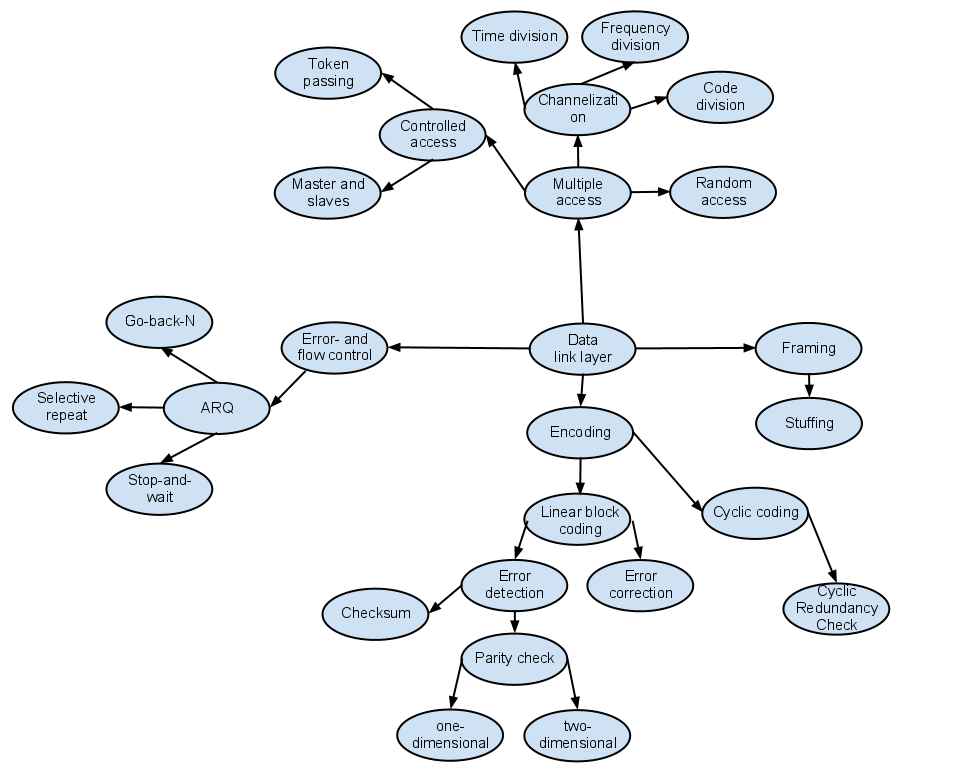
\includegraphics[scale=0.4,trim=0 0 0 0]{bobler_dll.png} %trim=l b r t (can cut off from every side)
	\caption{Things to consider concerning data link layer}
	\label{fig:bobler_dll}
	\end{center}
\end{figure}

\subsection{Encoding}
First thing to consider is the encoding of signals. Since there are sixteen
different DTMF combinations, each tone can carry four bits.

The only type of error to consider is the situation where a tone is
misinterpreted, which leads to a four bit burst error. Therefore the system
should be designed specifically to detect errors of this type. Since the media
is considered to be very noisy, transmissions should also be kept as short as
possible.

A two dimensional parity check will be able to detect burst errors of the
proposed size, so this is the choice. Implementing the parity check as a
four-by-four matrix will make it possible to transfer two bytes with a frame of
three bytes.

Example: We want to transmit the two bytes 0011 0101 and 0101 1110. The data
link layer puts these in a four by four matrix and calculates the parity bits by
adding the rows and columns:

\begin{table}[htb]
	\begin{center}
	\begin{tabular}{c|c}
	0011 & 0 \\
	0101 & 0 \\
	0101 & 0 \\
	1110 & 1 \\
	\hline
	1101 & \\
	\end{tabular}
	\end{center}
	\caption{Two-dimensional parity check}
	\label{tab:Two_dimensional_parity_check}
\end{table}

Instead of as normally done to increase the size of each row by one to contain
the parity bit, the parity bits are transmitted together as a redundant byte. In
the case of this example the transmission would be:

\begin{table}[htb]
	\begin{center}
	\begin{tabular}{c|c|c|c|c|c}
	0011 & 0101 & 0101 & 1110 & 0001 & 1101 \\
	\end{tabular}
	\end{center}
	\caption{Bytes to be transmitted}
	\label{tab:Bytes_to_be_transmitted}
\end{table}

Each four bit nipple is now transmitted an a DTMF-tone. Should one of the tones
be misinterpreted, the receiving data link layer would get a mismatch of the
parity bits for example:

\begin{table}[htb]
	\begin{center}
	\begin{tabular}{c|c}
	0011 & 0 \\
	0101 & 0 \\
	0000 & 0 \\
	1110 & 1 \\
	\hline
	1000 & \\
	\end{tabular}
	\end{center}
	\caption{Failed parity check}
	\label{tab:Failed_parity_check}
\end{table}

This will lead to the frame being discarded. Though in some cases it will be
possible to correct the error and find the original nibble, this is not
recommended, since more than one tone might be corrupted. Errors in the
redundant byte will also lead to the discarding of the transmission.

\subsection{Flowcontrol}
The next thing to consider is flowcontrol. Since the DTMF-system
cannot be used as full-duplex, piggybacking is impossible. This means that at
some point the receiver must reply. This reply will also be of six-tones, and
therefore it might as well contain information about witch frames to resend. In
other words a selective repeat system is preferred

To introduce a selective repeat system, additional redundancy is needed.

By using only two bits for the sequence number, redundancy is kept as low as
possible while still benefiting from pipelining. The sender transmits four
frames (twentyfour tones) and then waits for the receiver to reply with one frame (six
tones).

\subsection{Framing}
It is presumed that the physical layer will provide a starting point for each
transmission, probably in the form of silence. If this is not the case,
additional flags will be needed in between the frames, again leading to the need
of stuffing.

Next thing to consider is multipoint. There are three options: A token
network, a time division network or a code division network. Time division
requires a level of timing the interface layer is not able to deliver.
Code division leads to the need for larger frames or if implemented with the
proposed frame size, a lot of unused frames in a small network. This leaves us
with a token passing network, so this is the choice.

Four bits will control the adressing. The first two
bits identifies the receiver and the next two identifies the sender. Thereby the
protocol allows networks of up to four stations.

The selective repeat system and the token network introduces the need for different frame types.
The type field will consist of two bits, at the same time controlling
the token and indicating frame types. Rules must be implemented to keep the token circulating.

\begin{table}[htb]
	\begin{center}
	\begin{tabular}{|c|ll|}
		\hline
		00 & Has no token & Reply from receiver \\
		\hline
		01 & Has no token & Passes token to receiveradress \\
		\hline
		10 & Has token & Accepts token from receiveradress \\
		\hline
		11 & Has token & Data frame for receiveradress \\
		\hline
	\end{tabular}
	\end{center}
	\caption{Protocol for type field}
	\label{tab:Protocol_for_type_field}
\end{table}

This leads to the following format of a frame: 

\begin{table}[htb]
	\begin{center}
	\begin{tabular}{|ccc|c|c|}
		\hline
		type (2 bits) & address (4 bits) & sequence (2 bits) & data (8 bits) & parity (8 bits)  \\
		\hline
	\end{tabular}
	\end{center}
	\caption{Final frame format}
	\label{tab:Final_frame_format}
\end{table}



\chapter{Discussion}
Discussion

\chapter{Conclusion}
Conclusions are good

 
 
 

% References
\clearpage
\nocite{*} % Inkluderer alle poster i bibl.bib-filen (dvs. kun skriv litteratur ind vi rent faktisk har brugt)
\printbibliography
\addcontentsline{toc}{chapter}{Bibliography}


% Appendix
\appendix %all sections below are numbered ''A, B, C,...''
\chapter{Appendix section here}
Jaa

\end{document}